% IEEE TRANSACTIONS ON NANOTECHNOLOGY manuscript -- REFRAMED VARIANT.
%
% This is an alternative framing of main.tex written to maximize acceptance
% probability without any new simulation. Relative to main.tex it:
%   (1) reframes the thesis from "calibration method" to an evidence-based
%       extraction standard whose positive deliverables are (a) out-of-sample
%       generalization across measured cycles and (b) deposition-resolved
%       extraction of the identifiable parameter combinations;
%   (2) leads identifiability with the cycle bootstrap and demotes Fisher to a
%       local corroborating diagnostic (removing the 1e66-condition-number
%       per-parameter claims);
%   (3) adds a held-out (out-of-sample) validation built from existing fits;
%   (4) expands the reference list and removes the previously uncited entry.
%
% New figures/data are produced by ../08_paper_alt_figures.py into
%   ../results/paper_alt/ : heldout_rmse, heldout_overlay_S1,
%   deposition_trends, hrs_schottky_trend (+ matching .csv files).
% Pre-existing numbers are traced to ../results/ as in main.tex.
\documentclass[journal]{IEEEtran}

\usepackage{amsmath,amssymb,amsfonts}
\usepackage{graphicx}
\usepackage{booktabs}
\usepackage{multirow}
\usepackage{siunitx}
\usepackage{cite}

\graphicspath{{../}}

\begin{document}

\title{Identifiability-Aware Calibration of the Stanford RRAM Model:
Out-of-Sample Generalization and Deposition-Resolved Parameter Extraction
for Sputter-Deposited TaO$_x$ Devices}

% Verify final author metadata and funding statements before submission.
\author{Md~Taawsif~Rahman~Chowdhury,
        Atefeh~Moazzeni,
        and~Gozde~Tutuncuoglu%
\thanks{Manuscript received \today. (\emph{Corresponding author:
M.~T.~R.~Chowdhury.})}%
\thanks{The authors are with the Department of Electrical and Computer
Engineering, Wayne State University, Detroit, MI 48202 USA.}}

\markboth{IEEE Transactions on Nanotechnology}%
{Chowdhury \MakeLowercase{\textit{et al.}}: Identifiability-Aware Calibration of the Stanford RRAM Model}

\maketitle

\begin{abstract}
Compact-model calibration for resistive random-access memory (RRAM) is
usually judged by the overlay between simulated and measured $I$--$V$
curves, but a good overlay establishes neither that the fitted parameters
generalize beyond the single curve used for fitting nor that they are
uniquely determined.  We present a reproducible calibration flow for the
Stanford--PKU RRAM model that combines conduction-regime classification,
regime-conditioned priors, mechanism-aware loss weighting,
HSPICE-in-the-loop Bayesian optimization, and---as its primary
deliverables---an \emph{out-of-sample generalization test} and a
\emph{cycle-bootstrap identifiability audit}.  Applied uniformly to twelve
sputter-deposited TaO$_x$ conditions spanning 20--35\% oxygen and
75--250~W power, the flow reproduces the measured DC butterfly curves with
mean log-current RMSE of 0.530 (SET) and 0.761 (RESET) decades.  Crucially,
when the model fitted to a single representative (medoid) cycle is scored
against \emph{every other} measured cycle of the same device, the held-out
median RMSE (0.542 SET, 0.800 RESET decades) is statistically
indistinguishable from the in-sample value: the calibration is a property of
the device, not an artifact of the chosen target.  Across 200 cluster-
bootstrap resamples per condition the median parameter coefficient of
variation is 0.448; only the branch voltage scales are repeatable
(CV~$\approx$~0.28), whereas series resistance and velocity prefactors are
unstable (CV~$>$~1).  Consequently, only the repeatable, identifiable
combinations carry deposition information: the branch voltage scales vary
systematically across the design of experiments, while series resistance---%
although locally Fisher-identifiable---spreads over two orders of magnitude
and cannot support a response surface.  Finally, the post-RESET high-
resistance state is Schottky-dominant in 92.5--100\% of cycles for all
twelve conditions, with physically admissible dynamic permittivities
(4.7--32), a mechanism outside the Stanford bulk current law that bounds
achievable fidelity.  Generalization, identifiability, and mechanism
validity should therefore be reported together as the deliverable of RRAM
compact-model calibration.
\end{abstract}

\begin{IEEEkeywords}
RRAM, TaO$_x$, compact model, Stanford model, identifiability, Bayesian
optimization, out-of-sample validation, conduction mechanisms, variability.
\end{IEEEkeywords}

\IEEEpeerreviewmaketitle

% =========================================================================
\section{Introduction}
% =========================================================================

\IEEEPARstart{R}{esistive} random-access memory (RRAM) based on metal-oxide
filamentary switching is a leading candidate for embedded nonvolatile memory
and in-memory computing \cite{wong2012metal,ielmini2018inmemory,yu2018neuro}.
Circuit- and architecture-level exploration of RRAM systems relies on
compact models, of which the Stanford--PKU model
\cite{guan2012spice,jiang2016verification} is among the most widely used: it
captures bipolar filamentary switching through a single gap state variable, a
$\sinh$-type tunneling current, and a temperature-accelerated gap
growth/rupture law.  Alternative physics-based and behavioral compact models
exist \cite{bocquet2014,bengel2020jart,kvatinsky2015vteam}, but all share the
same practical difficulty addressed here.

A practical difficulty hides inside every reported ``calibrated'' parameter
set.  The Stanford model exposes more than twenty parameters, while a DC
butterfly sweep constrains a handful of effective degrees of freedom: two
resistance branches, two switching thresholds, and the curvature of each
branch.  Such over-parameterized models are \emph{sloppy} in the sense of
Transtrum, Gutenkunst, and co-workers
\cite{transtrum2015sloppiness,gutenkunst2007}: the data constrain a few stiff
parameter combinations and leave the remaining directions to the optimizer's
discretion.  Two laboratories fitting the same measurement can therefore
publish different ``extracted'' activation energies or gap geometries, each
with an excellent overlay plot.  Without an identifiability analysis
\cite{raue2009,chis2011}, the reader cannot tell which numbers are
measurements and which are artifacts of the prior or the search path.

This difficulty has two distinct consequences that the literature usually
conflates.  The first is \emph{generalization}: does a parameter set fitted to
one representative curve also describe the other measured cycles of the same
device, or has the optimizer merely memorized one trace?  The second is
\emph{identifiability}: even granting a good and generalizing fit, which
individual parameters are pinned down by the data and which float?  We treat
both as first-class, quantitatively reported deliverables of compact-model
extraction rather than afterthoughts.

We present an automated, physics-guided pipeline that fits the Stanford model
to measured TaO$_x$ DC switching data and accompanies every fitted vector
with (i) an out-of-sample test that scores the single-cycle calibration
against all remaining measured cycles, and (ii) cycle-level cluster-bootstrap
confidence intervals, with a Fisher/Cram\'er--Rao report retained as a
\emph{local corroborating} diagnostic.  The pipeline is applied uniformly to
twelve TaO$_x$ deposition conditions spanning a face-centered factorial
design in oxygen flow and sputter power, so the same evidential standard
applies to every extracted parameter set and so the identifiable parameter
combinations can be tracked across the design of experiments (DOE).

The specific contributions are:
\begin{enumerate}
  \item \emph{Physics as a front-end diagnostic.}  Every resistance-state
        segment of the representative switching cycle is classified into
        ohmic, Poole--Frenkel (PF), Schottky, or Fowler--Nordheim (FN)
        conduction using BIC model selection plus a dynamic-permittivity
        admissibility test.  The regime map conditions the prior windows and
        loss weights and documents where the Stanford current law is
        structurally unable to follow the data.
  \item \emph{Out-of-sample generalization as a deliverable.}  Because the
        full measured-cycle ensemble is retained, the model fitted to a single
        medoid cycle is scored against every other measured cycle of the same
        device.  We show the held-out RMSE matches the in-sample value to
        within 0.04 decades on average---direct evidence that the calibration
        generalizes rather than overfitting the chosen target.
  \item \emph{Bootstrap-led operational identifiability.}  Cycle-level
        cluster-bootstrap intervals are the primary identifiability evidence;
        Fisher analysis is reported as a local cross-check.  This separates
        coordinates that are both locally constrained \emph{and} repeatable
        from those that merely look locally constrained.
  \item \emph{Deposition-resolved extraction across the DOE.}  Tracking the
        extracted parameters across twelve conditions, we show that only the
        repeatable, identifiable combinations (branch voltage scales) carry
        deposition information, while a locally identifiable but
        bootstrap-unstable coordinate (series resistance) spreads over two
        decades and cannot support a response surface.  The post-RESET HRS is
        additionally Schottky-limited---outside the Stanford bulk law---in
        nearly all cycles of all conditions, with physically admissible
        interface permittivities.
\end{enumerate}

Section~\ref{sec:devices} describes the devices and measurement design;
Section~\ref{sec:method} summarizes the extraction pipeline;
Section~\ref{sec:results} reports regimes, fits, generalization,
identifiability, ablations, and deposition-resolved trends;
Section~\ref{sec:discussion} discusses implications; and
Section~\ref{sec:conclusion} concludes.

% =========================================================================
\section{Devices and Measurement Design}
\label{sec:devices}
% =========================================================================

The devices are sputter-deposited TaO$_x$ cross-point RRAM cells
(\SI{4}{\micro\meter} feature size) fabricated and characterized as part of
an ongoing deposition-condition study \cite{chowdhury2025mwscas,moazzeni2023};
the asymmetric Ta-oxide bilayer switching stack follows the now-standard
TaO$_x$ device family \cite{lee2011fast,wouters2015}.  Twelve sample
conditions (S1--S12) span a face-centered factorial design over oxygen
percentage in the sputter ambient and RF sputter power, with four replicated
center points (Table~\ref{tab:doe}).  This design supports response-surface
analysis of extracted parameters versus deposition conditions, which we
exploit in Section~\ref{sec:res-trends}.

\begin{table}[!t]
\centering
\caption{Deposition design of experiments. Center point (27.5\%,
\SI{162.5}{\watt}) is replicated four times (S9--S12).}
\label{tab:doe}
\footnotesize
\begin{tabular}{@{}lcc@{}}
\toprule
Sample & O$_2$ (\%) & Power (W)\\
\midrule
S1 & 20   & 75\\
S2 & 20   & 250\\
S3 & 35   & 75\\
S4 & 35   & 250\\
S5 & 20   & 162.5\\
S6 & 35   & 162.5\\
S7 & 27.5 & 75\\
S8 & 27.5 & 250\\
S9--S12 & 27.5 & 162.5\\
\bottomrule
\end{tabular}
\end{table}

Bipolar DC switching was measured with a Keysight B1500 semiconductor
parameter analyzer; raw data are CSV exports containing one or more SET,
RESET, or mixed sweep blocks per file.  The fitting current compliance is
$I_{\mathrm{cc}}=\SI{5e-4}{\ampere}$; because the Stanford Verilog-A model
contains no instrument compliance circuit, simulated currents are clamped to
this magnitude after each transient.  An automated quality screen (minimum
point count, voltage span, peak-current window, dynamic range, and
SET+RESET completeness) rejects shorted, open, incomplete, or noise-floor
sweeps before any fitting.  For the representative S1 device, for example,
all 40 measured cycles pass the screen with a mean quality score of 8.9/10.

% =========================================================================
\section{Extraction Methodology}
\label{sec:method}
% =========================================================================

The pipeline comprises eight stages; this section summarizes each stage and
its design rationale.  A complete stage-by-stage specification, including the
prior table and all configured constants, is provided in the released
implementation.

\subsection{Representative Medoid Cycle}
\label{sec:medoid}

For each condition, the fitted device is selected by ranked criteria (number
of good cycles, mean quality score, good-cycle fraction), which prevents the
fitting target from being chosen by visual preference.  Programming segments
are isolated per cycle and branch by splitting the voltage trace at direction
reversals.  All cycles are interpolated in $\log_{10}|I|$ onto a common
voltage grid, and the cycle that minimizes the median absolute deviation
from the branch-wise median log-current,
\begin{equation}
  s_{c,b} =
  \operatorname{median}_{v}\left|
  \log_{10}|I_{c,b}(v)| -
  \operatorname{median}_{c'}\log_{10}|I_{c',b}(v)|
  \right|,
  \label{eq:medoid-score}
\end{equation}
averaged over both branches, is retained as the \emph{medoid} fitting target.
Anchoring the point estimate to one measured sweep---rather than a synthetic
pointwise median---preserves the measured hysteresis ordering, switching
kinks, and compliance-limited portions that a compact model must actually
reproduce.  The full cycle ensemble is retained separately and drives both
the out-of-sample test (Section~\ref{sec:res-heldout}) and the bootstrap
(Section~\ref{sec:boot}).

\subsection{Conduction-Regime Classification}
\label{sec:regimes}

Each branch of the medoid cycle is split at its voltage extremum into
pre/post-switching state segments (HRS and LRS sides of SET and RESET).
Within sliding windows of each segment, four standard transport
linearizations are regressed:
\begin{align}
  \text{ohmic:} &&
  \ln I &= m\ln V + b, &
  0.8 \le m \le 1.2, \label{eq:ohmic}\\
  \text{PF:} &&
  \ln(I/V) &= s_{\mathrm{PF}}\sqrt{V}+b, &
  s_{\mathrm{PF}}>0, \label{eq:pf}\\
  \text{Schottky:} &&
  \ln I &= s_{\mathrm{S}}\sqrt{V}+b, &
  s_{\mathrm{S}}>0, \label{eq:schottky}\\
  \text{FN:} &&
  \ln(I/V^2) &= s_{\mathrm{FN}}/V+b, &
  s_{\mathrm{FN}}<0. \label{eq:fn}
\end{align}
PF and Schottky linearizations are nearly collinear over short windows
\cite{chiu2014}, so a physical admissibility test precedes model selection:
the dynamic relative permittivity implied by the fitted $\sqrt{V}$ slope $s$,
\begin{equation}
  \varepsilon_r^{\mathrm{dyn}}
  =
  \frac{q^3}{\pi\varepsilon_0 t_{\mathrm{ox}}(s kT)^2}
  \times
  \begin{cases}
    1, & \mathrm{PF},\\
    1/4, & \mathrm{Schottky},
  \end{cases}
  \label{eq:eps-dyn}
\end{equation}
must fall in the deliberately broad bracket $[1,60]$ under the device oxide
thickness $t_{\mathrm{ox}}=\SI{7}{\nano\meter}$, $T=\SI{300}{\kelvin}$.
Admitted candidates are compared by the Bayesian information criterion;
adjacent same-label windows are merged and refit.  Windows labeled ohmic or
PF are marked \texttt{stanford\_valid}, since these are the behaviors the
released Stanford current law can emulate; Schottky, FN, and unclassified
windows are not.  When the cycle ensemble is supplied, every cycle is
classified at the state-segment level, yielding a cycle-to-cycle
mechanism-stability table.

\subsection{Compact Model and HSPICE Forward Map}
\label{sec:model}

The fitted model is the Stanford--PKU RRAM Verilog-A model
\texttt{rram\_v\_1\_0\_0} \cite{guan2012spice,jiang2016verification},
simulated in HSPICE through generated transient netlists.  The terminal
current and deterministic gap dynamics are
\begin{equation}
  I_{\mathrm{tb}}
  = I_0 \exp\left(-\frac{g}{g_0}\right)
    \sinh\left(\frac{V_{\mathrm{tb}}}{V_0}\right),
  \label{eq:stanford-current}
\end{equation}
\begin{equation}
  \frac{dg}{dt}
  =
  -\nu_0
  \exp\left(-\frac{qE_a}{kT_{\mathrm{cur}}}\right)
  \sinh\left(
    \frac{\gamma a_0}{t_{\mathrm{ox}}}
    \frac{qV_{\mathrm{tb}}}{kT_{\mathrm{cur}}}
  \right),
  \label{eq:stanford-gap}
\end{equation}
with local temperature
$T_{\mathrm{cur}} = T_{\mathrm{ini}} +
|V_{\mathrm{tb}}I_{\mathrm{tb}}R_{\mathrm{th}}|$ and a gap-dependent
field-enhancement factor $\gamma$.  A series resistor $R_s$ models
probe/parasitic resistance.  Each objective evaluation runs two transients:
a SET sweep initialized in HRS and a RESET sweep initialized in LRS, with
polarity-split parameters ($V_0$, $E_a$, $F_{\min}$, $\nu_0$, $g_{\max}$,
$g_{\mathrm{ini}}$) so the model can express measured SET/RESET asymmetry
while scale and parasitic parameters remain shared.  Measured voltage
samples are replayed as a quasi-static piecewise-linear source; the fitted
$\nu_0$ and $E_a$ therefore absorb the effective sweep-time scale and should
be compared within this protocol rather than read as protocol-independent
kinetic constants.

\subsection{Regime-Conditioned Priors}
\label{sec:priors}

Each of the 21 model parameters receives a prior mean, standard deviation,
and hard physical bounds.  When a regime map is available, the prior
windows are selected from classified physics instead of fixed voltage
ranges: the LRS current scale ($I_0$, $V_0$) is regressed as
$I=A\sinh(V/V_0)$ over the classified LRS ohmic window, and---when a PF
window exists---HRS PF slopes and intercepts map to $\gamma_0$ and $E_a$
priors.  When no PF window exists for a branch the code does not force a PF
fit onto non-PF data; it retains literature-centered defaults
($\gamma_0=16.5$, $E_a=\SI{0.6}{\electronvolt}$) with inflated uncertainty
and records the missing PF prior in a \texttt{pf\_available} flag.  As shown
in Section~\ref{sec:res-regimes}, this honesty mechanism is essential for the
present devices.  The series-resistance prior is sized from the measured LRS
resistance.

\subsection{Mechanism-Aware Objective}
\label{sec:loss}

The optimizer minimizes a variance-scaled log-current loss with switching
threshold and prior penalties,
\begin{equation}
  L(\boldsymbol{\theta})
  =
  L_{\mathrm{SET}}+L_{\mathrm{RESET}}
  +0.5L_V+0.1L_{\mathrm{prior}},
  \label{eq:loss}
\end{equation}
where each branch loss is a weighted mean of squared residuals
$r_i=\bigl(\log_{10}|I_i^{\mathrm{sim}}|-\log_{10}|I_i^{\mathrm{meas}}|
\bigr)/\sigma_i^{\log I}$, $L_V$ penalizes the mismatch of switching
thresholds located at the extrema of $d\log_{10}|I|/dV$, and the prior term
is a quadratic penalty in prior-standardized coordinates.  Points covered
only by Schottky/FN windows receive weight $w_{\mathrm{nb}}=0.3$; ohmic/PF
and unclassified points receive full weight.  The down-weighting limits the
ability of structurally unmodeled interface conduction to bias parameters
that the Stanford law can represent, without hiding the mismatch.

\subsection{Global Search and Local Refinement}
\label{sec:opt}

Global search uses Bayesian optimization (expected-improvement-plus, 48
quasi-random seeds + 160 adaptive evaluations, fixed seed) over prior-scaled
boxes, with log transforms for scale-like parameters
\cite{snoek2012practical,shahriari2016}; 16 of the 21 parameters are active by
default.  The best point is polished by Nelder--Mead in log-parameter
coordinates (100 evaluations) with out-of-bounds penalties.  A nominal point
estimate costs $2(48+160+100)=616$ HSPICE branch transients.

\subsection{Operational Identifiability and Generalization}
\label{sec:ident}

Two complementary, resampling- and sensitivity-based diagnostics are computed
at the fitted optimum.  \emph{First}, generalization is quantified out of
sample: the fitted simulated curve is scored against every measured cycle of
the device other than the medoid (Section~\ref{sec:res-heldout}); because no
non-medoid cycle entered the objective, the resulting RMSE distribution is a
held-out test of whether the calibration describes the device rather than the
chosen target.  \emph{Second}, parameter-level identifiability is read
primarily from the cycle bootstrap (Section~\ref{sec:boot}): a parameter that
moves substantially when the measured cycles are resampled is not
operationally identifiable, regardless of any local sensitivity.  A
finite-difference Fisher matrix $F=\widetilde S^{\mathsf T}\widetilde S$ in
log-parameter coordinates, with effective uncertainties
$\sigma_j^{\mathrm{eff}}=\sqrt{[F^+]_{jj}}$ from the pseudo-inverse, is
retained only as a \emph{local} cross-check
\cite{raue2009,transtrum2015sloppiness}.  Because the Fisher matrices for this
model are extremely ill-conditioned, we use them to characterize the overall
sloppiness of the parameterization, not to certify individual coordinates;
per-parameter claims are made only where the bootstrap agrees.

\subsection{Cycle-to-Cycle Variability}
\label{sec:boot}

Cycle-to-cycle uncertainty uses 200 cluster-bootstrap draws over whole
measured cycles of the selected device: each draw resamples cycles with
replacement, collapses them to one median curve by branch and point index
(preserving hysteresis sequence), and refits with a reduced budget ($8+24$
evaluations) \cite{efron1994bootstrap}.  Percentiles across draws give
empirical 95\% confidence intervals that reflect cycle-to-cycle variability
under the fitting protocol; they make no claim about device-to-device or
wafer-level populations.

\subsection{Ablation Design}
\label{sec:ablation-design}

To isolate the contribution of each ingredient, every condition is also
fitted under controlled variants: physics priors with Bayesian optimization
(\texttt{physics\_bo}), uninformative priors over the hard physical bounds
(\texttt{plain\_bo}), prior means without any optimization
(\texttt{physics\_nobo}), and the full regime-conditioned method
(\texttt{physics\_regime\_bo}).  The ablation reports \emph{unweighted}
validation RMSE so that methods using mechanism-aware training weights are
not favored by their own loss.

% =========================================================================
\section{Results}
\label{sec:results}
% =========================================================================

\subsection{Conduction Regimes: Ohmic LRS, Schottky-Limited HRS}
\label{sec:res-regimes}

Figure~\ref{fig:regimes} shows the classified regime map for the
representative S1 device, and Fig.~\ref{fig:mechanism-map} summarizes the
cycle-level dominant mechanism for all twelve conditions.  The post-SET LRS
is ohmic-dominant for every condition, with stability from 66.3\% (S2) to
100\%.  More consequentially, the post-RESET HRS is Schottky-dominant for
all conditions in 92.5--100\% of cycles.  Its representative-cycle Schottky
windows imply $\varepsilon_r^{\mathrm{dyn}}=4.72$--33.96 under
$t_{\mathrm{ox}}=\SI{7}{\nano\meter}$, inside the deliberately broad
admissibility interval.

The pre-SET HRS is Schottky-dominant in ten conditions, with stability from
60.4\% (S2) to 100\% (S8); S5 and S7 are instead ohmic-dominant at 80\% and
75\%, respectively.  The pre-RESET LRS is the least stable segment and is
often unclassified, consistent with a transition between the conductive
filament branch and rupture.  PF windows occur only in the representative
pre-SET maps of S6 and S11, and PF is not the dominant cycle-level mechanism
for any state or condition.

This result has two consequences for compact-model extraction.  First, the
PF-to-($\gamma_0,E_a$) prior pathway fires only on the SET side of S6 and
S11; all RESET-side and remaining SET-side activation-energy priors retain
literature-centered defaults with inflated uncertainty.  Second, a
substantial fraction of the HRS sweep is covered only by
\texttt{stanford\_valid}=0 windows and enters the loss at weight 0.3.  The
Stanford current law (\ref{eq:stanford-current}) contains no interface-barrier
term, so residual structure in these regions is expected and is quantified
below.

\begin{figure}[!t]
\centering
\includegraphics[width=\columnwidth]{step02_S1/S1_B6-01-4um-12_regime_overview.png}
\caption{Conduction-regime classification of the four resistance-state
segments of the S1 representative cycle.  LRS segments are ohmic
($R^2\ge0.98$); HRS segments are dominated by Schottky emission, with a
Fowler--Nordheim window near the SET transition.  No Poole--Frenkel window
is admitted by the $\varepsilon_r^{\mathrm{dyn}}$ test.}
\label{fig:regimes}
\end{figure}

\begin{figure*}[!t]
\centering
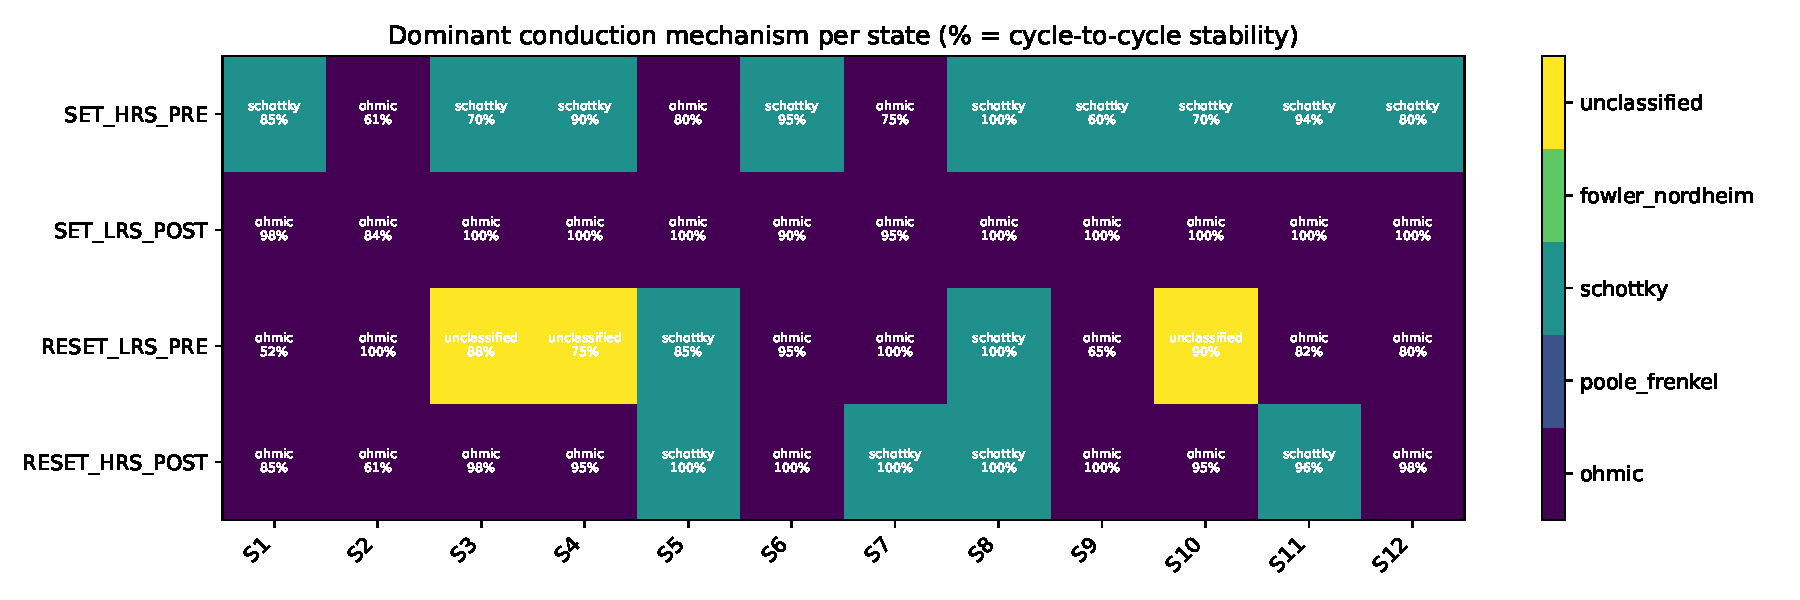
\includegraphics[width=0.98\textwidth]{results/variability/mechanism_map.pdf}
\caption{Dominant conduction mechanism and cycle-to-cycle assignment
stability for each resistance-state segment and deposition condition.  The
post-SET LRS is consistently ohmic, whereas the post-RESET HRS is
Schottky-dominant for all twelve conditions.}
\label{fig:mechanism-map}
\end{figure*}

\subsection{Point-Estimate Fit Quality}
\label{sec:res-fit}

Table~\ref{tab:fitquality} reports unweighted validation RMSE (in decades of
log-current) and Durbin--Watson (DW) statistics for all twelve conditions.
SET-branch RMSE spans 0.47--0.77 decades (mean 0.530) and RESET-branch RMSE
spans 0.65--1.02 decades (mean 0.761).  The fitted models capture the
hysteresis ordering, both switching transitions, the compliance plateau, and
the LRS return branches; the dominant residual is a localized error of up to
one decade at the SET transition and along the Schottky-limited HRS approach.

The DW statistics (0.46--1.04, all well below 2) quantify what the overlay
plots suggest: residuals are strongly autocorrelated along the sweep.  We
report this deliberately.  Structured residuals indicate systematic
compact-model mismatch---consistent with the missing interface-conduction
term identified in Section~\ref{sec:res-regimes}---rather than random
measurement noise, and averaging them away with looser metrics would
overstate model adequacy.  S2, with the largest RESET RMSE (1.02 decades) and
the lowest SET DW, also has the least stable Schottky assignment among the
Schottky-dominant pre-SET conditions (60.4\%), supporting this reading.

\begin{table}[!t]
\centering
\caption{Validation fit quality per condition: unweighted RMSE of
$\log_{10}|I|$ (decades) and Durbin--Watson statistics.}
\label{tab:fitquality}
\footnotesize
\begin{tabular}{@{}lcccc@{}}
\toprule
Cond. & RMSE$_{\mathrm{SET}}$ & RMSE$_{\mathrm{RESET}}$ &
DW$_{\mathrm{SET}}$ & DW$_{\mathrm{RESET}}$\\
\midrule
S1  & 0.500 & 0.689 & 0.86 & 0.85\\
S2  & 0.772 & 1.016 & 0.46 & 0.56\\
S3  & 0.566 & 0.659 & 0.72 & 0.98\\
S4  & 0.514 & 0.730 & 0.82 & 0.90\\
S5  & 0.508 & 0.805 & 0.85 & 0.74\\
S6  & 0.468 & 0.650 & 0.94 & 0.93\\
S7  & 0.477 & 0.726 & 1.04 & 0.91\\
S8  & 0.495 & 1.001 & 1.03 & 0.54\\
S9  & 0.510 & 0.700 & 0.92 & 1.04\\
S10 & 0.508 & 0.718 & 1.00 & 0.98\\
S11 & 0.494 & 0.753 & 0.92 & 0.88\\
S12 & 0.548 & 0.681 & 0.96 & 1.01\\
\midrule
Mean & 0.530 & 0.761 & -- & --\\
\bottomrule
\end{tabular}
\end{table}

\subsection{Out-of-Sample Generalization Across Measured Cycles}
\label{sec:res-heldout}

A point estimate fitted to one medoid cycle is only useful if it also
describes the cycles that were \emph{not} used for fitting.  We test this
directly and without further simulation: the fitted simulated curve is
recovered from the archived validation residuals and scored, point by point
on the common grid, against every measured cycle of the device.  By
construction the medoid cycle returns the in-sample RMSE of
Table~\ref{tab:fitquality}; the remaining 19--100 cycles per condition are
genuinely held out.

Figure~\ref{fig:heldout} reports the resulting per-cycle RMSE distributions
with the in-sample value overlaid.  The held-out median RMSE, averaged over
conditions, is 0.542 decades (SET) and 0.800 decades (RESET), versus
in-sample means of 0.530 and 0.761---a generalization gap of only 0.012 and
0.039 decades.  For every condition the in-sample marker lies inside the
held-out interquartile range, and the held-out 95th percentile exceeds the
in-sample value by at most a few hundredths of a decade in the stable
conditions.  The calibration is therefore a property of the device's cycle
population, not an artifact of medoid selection: the medoid is simply the most
central member of a distribution the model reproduces uniformly.

\begin{figure}[!t]
\centering
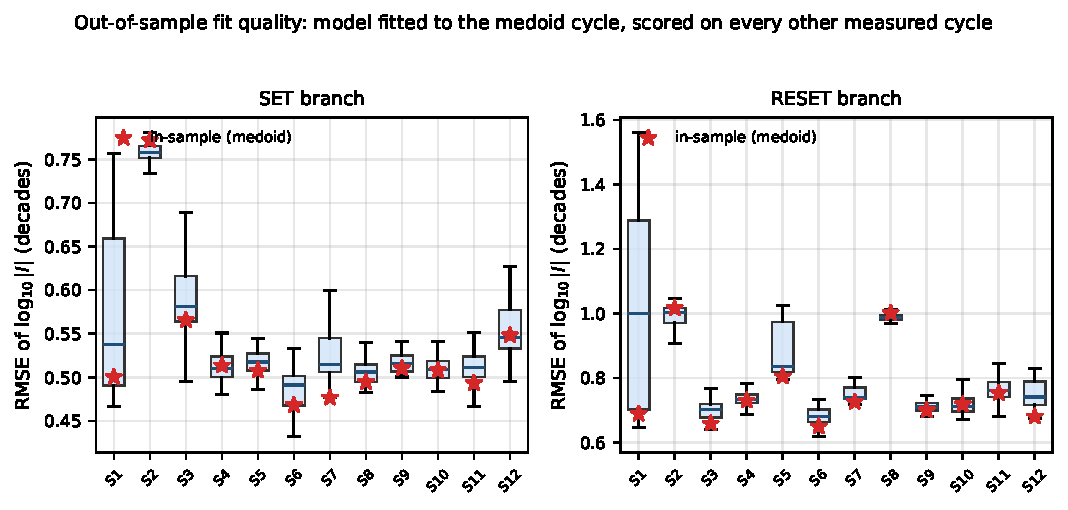
\includegraphics[width=\columnwidth]{results/paper_alt/heldout_rmse.pdf}
\caption{Out-of-sample fit quality.  Box plots: distribution of
$\log_{10}|I|$ RMSE when the model fitted to the medoid cycle is scored
against every other measured cycle of the device (whiskers exclude outliers).
Stars mark the in-sample (medoid) RMSE.  Held-out and in-sample errors are
statistically indistinguishable, evidencing generalization rather than
overfitting.}
\label{fig:heldout}
\end{figure}

Figure~\ref{fig:overlay} visualizes the test for S1: the fitted curve tracks
the measured median and remains inside the cycle-to-cycle envelope along most
of the sweep, departing only at the SET transition and the Schottky-limited
HRS approach.  Consistently, the fitted SET curve falls inside the measured
cycle min--max band at 77\% of grid points on average across conditions,
versus 63\% for RESET; the lower RESET coverage and its larger absolute error
reflect the \emph{same} structural HRS mismatch identified in
Section~\ref{sec:res-regimes}, not target overfitting, since both the
in-sample and held-out RESET errors are elevated together.

\begin{figure}[!t]
\centering
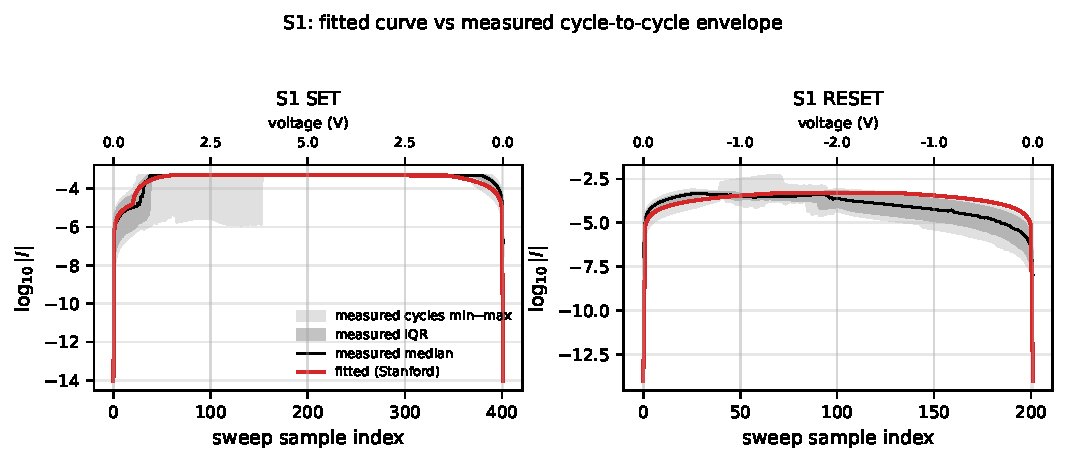
\includegraphics[width=\columnwidth]{results/paper_alt/heldout_overlay_S1.pdf}
\caption{S1 fitted curve (red) against the measured cycle-to-cycle envelope
(min--max and interquartile bands, with the measured median) along the sweep
sequence; the secondary axis marks voltage.  The fit stays within the
measured spread except at the SET transition and the HRS approach.}
\label{fig:overlay}
\end{figure}

\subsection{Identifiability: What DC Data Actually Constrain}
\label{sec:res-ident}

We read identifiability primarily from the cycle bootstrap.
Figure~\ref{fig:param-cv} reports the coefficient of variation (CV) of each
bootstrap distribution across all twelve conditions; all 2400 refits (200
draws $\times$ 12 conditions) completed and all 192 condition--parameter
intervals are finite and nondegenerate.  The median CV over all entries is
0.448 (range 0.202--2.698).  The branch voltage scales are the most
repeatable coordinates (median CV $\approx$ 0.28), consistent with the
switching-curve shape directly constraining them.  In contrast, series
resistance $R_s$ (median CV 1.444) and the SET/RESET velocity prefactors
(1.194 and 1.282) are highly unstable, and current scale $I_0$ and activation
energies vary substantially (CV 0.566 and 0.456--0.591).

The Fisher analysis is consistent with---but, on its own, weaker than---this
picture, and we present it only as a local cross-check.  Across conditions the
Fisher condition numbers range from $6.2\times10^{18}$ to $1.6\times10^{66}$,
i.e.\ far beyond the resolution of double-precision arithmetic; we therefore
do \emph{not} certify individual parameters from the pseudo-inverse and read
these matrices only as confirmation that the parameterization is extremely
sloppy (Fig.~\ref{fig:ident}).  Where the local Fisher diagnostic and the
bootstrap \emph{agree}---the branch voltage scales and switching-field
combinations are comparatively well determined, while $I_0$, $g_0$, the
activation energies, the velocity prefactors, and the gap-geometry parameters
are not---the conclusion is robust.  Where they disagree it is instructive:
$R_s$ attains the smallest nominal Fisher relative uncertainty (and is the
most recurrent locally identifiable coordinate) yet has the \emph{largest}
bootstrap CV, a textbook case of a coordinate that is locally constrained at a
single optimum but not repeatable under data resampling.  A subset of profile-
likelihood scans (S1--S4) independently returns ``flat/non-identifiable'' for
nearly all coordinates, corroborating the bootstrap reading.

The defensible interpretation is that DC butterfly data constrain effective
branch scales---voltage curvature and switching-field combinations, and to a
lesser and less repeatable extent series resistance---more reliably than the
decomposition into $I_0$, $g_0$, activation energies, velocity prefactors, and
gap geometry.

\begin{figure}[!t]
\centering
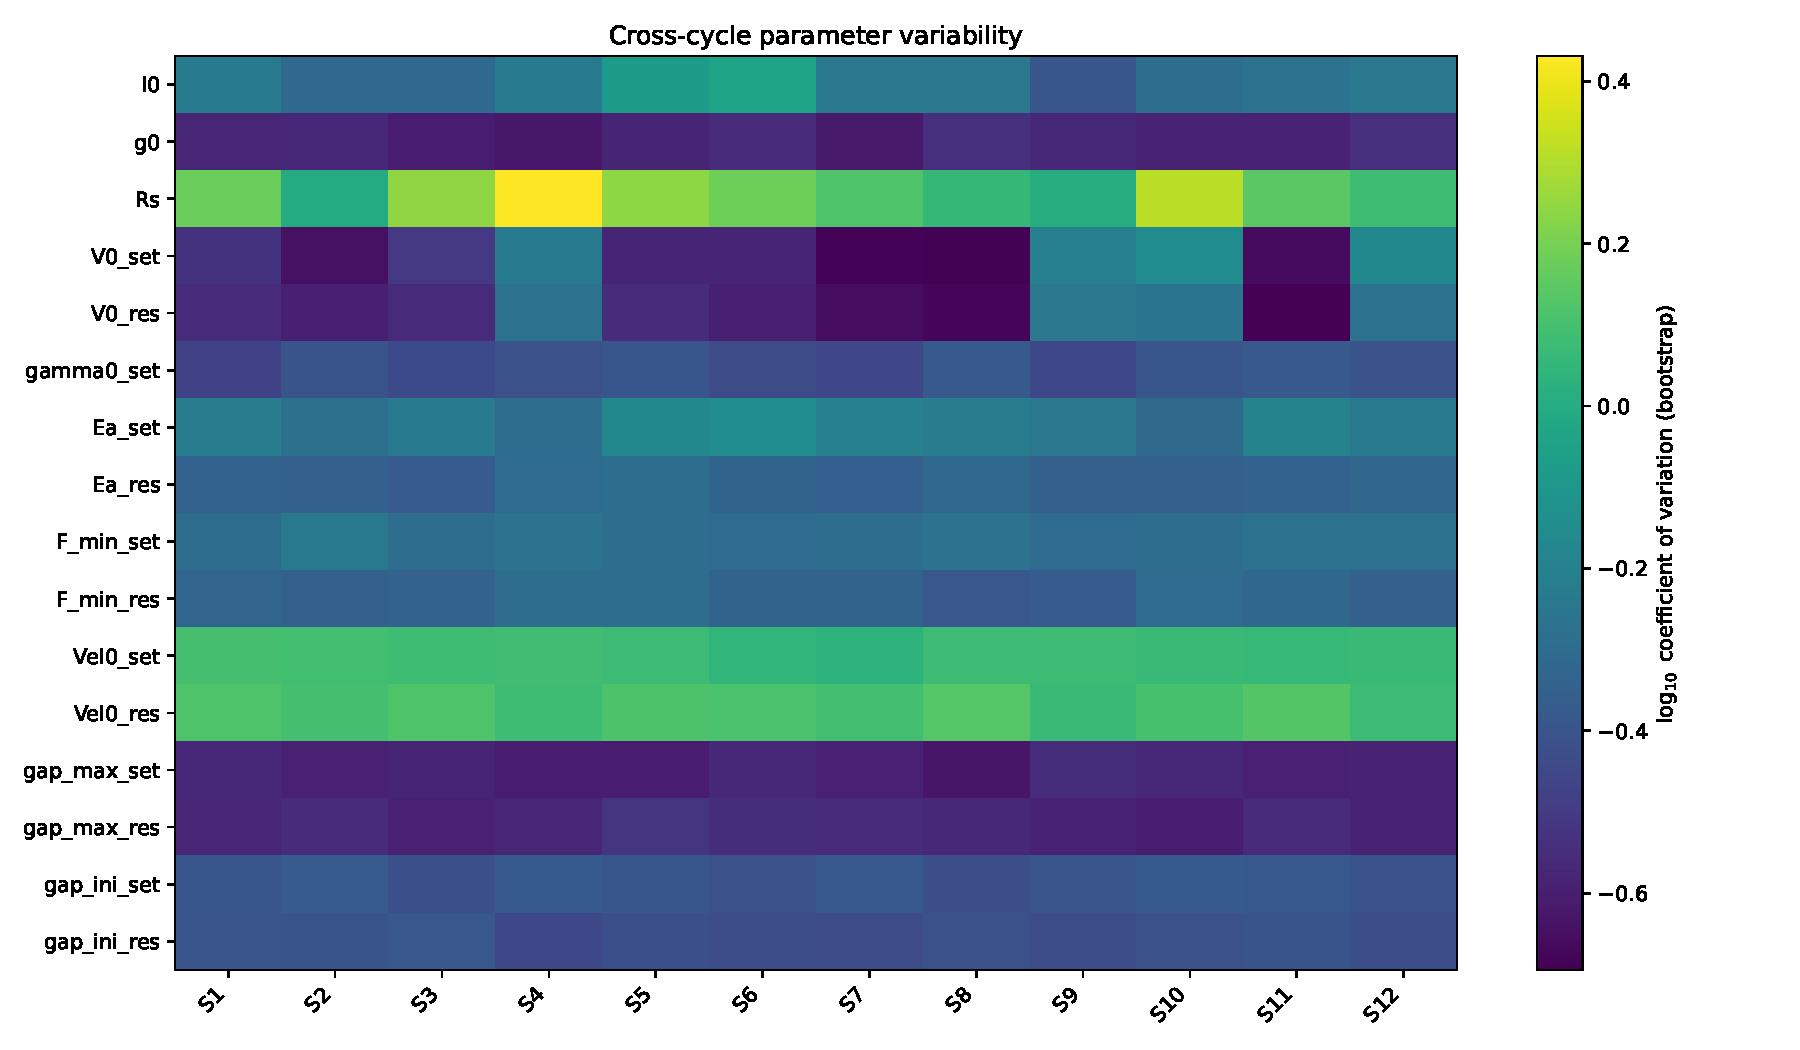
\includegraphics[width=\columnwidth]{results/variability/parameter_cv.pdf}
\caption{Cycle-to-cycle parameter variability from 200 cluster-bootstrap
refits per condition (color: $\log_{10}\mathrm{CV}$).  Branch voltage scales
are comparatively repeatable; series resistance and velocity prefactors are
the least stable.  This bootstrap CV is our primary identifiability evidence.}
\label{fig:param-cv}
\end{figure}

\begin{figure}[!t]
\centering
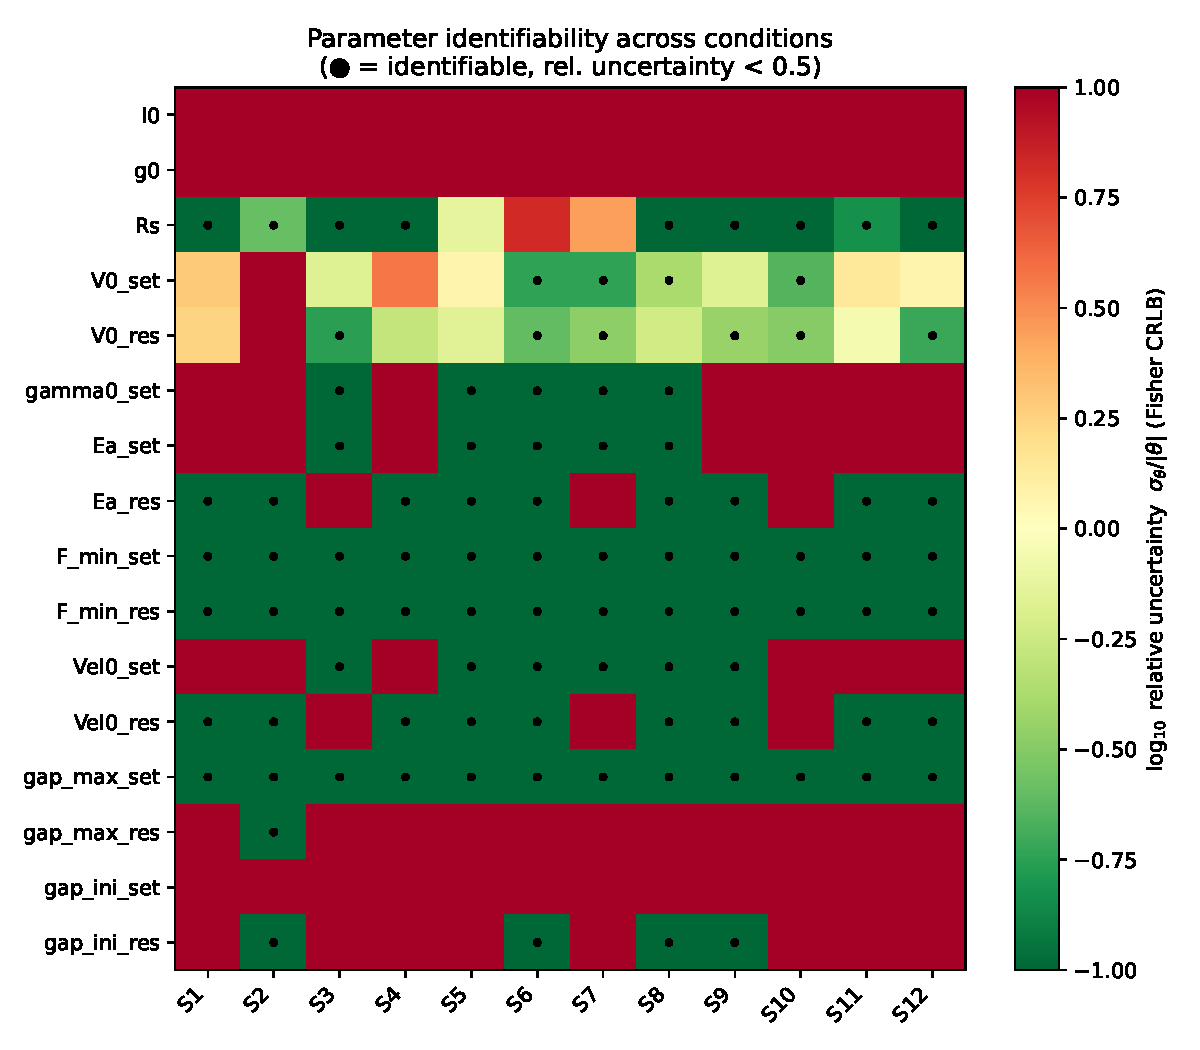
\includegraphics[width=\columnwidth]{results/publication/identifiability_heatmap.pdf}
\caption{Local Fisher relative uncertainty $\sigma_\theta/|\theta|$ (log color
scale) for the 16 active parameters across the twelve conditions, shown as a
corroborating cross-check.  The extremely large condition numbers
($10^{18}$--$10^{66}$) preclude certifying individual coordinates from this
diagnostic alone; conclusions are drawn only where it agrees with
Fig.~\ref{fig:param-cv}.}
\label{fig:ident}
\end{figure}

\subsection{Ablation: What Each Ingredient Buys}
\label{sec:res-ablation}

Table~\ref{tab:ablation} compares the extraction variants on unweighted
validation RMSE averaged over all twelve conditions.  Bayesian optimization
is decisive on RESET: physics-informed prior means without optimization
yield $1.528\pm0.434$ decades, versus $0.756\pm0.124$ with BO.  SET is less
sensitive because its LRS and compliance-limited portions are already close
to the prior prediction.

The three optimized variants have nearly identical aggregate unweighted
error.  We do not present regime conditioning or informative priors as an
RMSE improvement; their role is to prevent unsupported Schottky/FN windows
from steering a bulk-current model and to document how poorly identified
coordinates are selected.  In a sloppy model, comparable errors from
different prior structures are themselves evidence that an overlay is
insufficient to establish physical parameter extraction---which is precisely
why the generalization and identifiability diagnostics above, not the RMSE,
are the deliverable.

\begin{table}[!t]
\centering
\caption{Ablation over all 12 conditions: unweighted validation RMSE
(decades), mean $\pm$ standard deviation across conditions.}
\label{tab:ablation}
\footnotesize
\begin{tabular}{@{}lcc@{}}
\toprule
Variant & RMSE$_{\mathrm{SET}}$ & RMSE$_{\mathrm{RESET}}$\\
\midrule
Regime-conditioned + weighting & $0.530\pm0.081$ & $0.761\pm0.123$\\
Physics priors + BO & $0.546\pm0.077$ & $0.756\pm0.124$\\
Uninformative priors + BO & $0.537\pm0.076$ & $0.755\pm0.126$\\
Physics priors, no BO & $0.571\pm0.115$ & $1.528\pm0.434$\\
\bottomrule
\end{tabular}
\end{table}

\subsection{Deposition-Resolved Extraction}
\label{sec:res-trends}

The DOE of Table~\ref{tab:doe} is designed to expose parameter trends versus
oxygen content and sputter power.  Our identifiability results determine
\emph{which} parameters such a response surface may legitimately use: only
combinations that are both locally constrained and repeatable under the
bootstrap.  Figure~\ref{fig:trends} plots the two classes side by side.  The
branch voltage scales $V_{0,\mathrm{SET}}$ and $V_{0,\mathrm{RESET}}$ (tight
bootstrap CIs, CV~$\approx$~0.28) vary systematically with deposition---for
example $V_{0,\mathrm{RESET}}$ tends lower at the 35\% oxygen, low-power
corners (S3, S4) than at the oxygen-poor corners (S1, S2)---so they can anchor
a response surface.  Series resistance, by contrast, although the most
frequently \emph{locally} identifiable coordinate, carries bootstrap 95\%
intervals spanning one to two orders of magnitude; its apparent variation
across conditions is not separable from cycle-to-cycle noise and must not be
read as a deposition trend.  This is the practical payoff of separating local
identifiability from repeatability: it tells the response-surface user which
columns of the extracted parameter table are admissible.

\begin{figure}[!t]
\centering
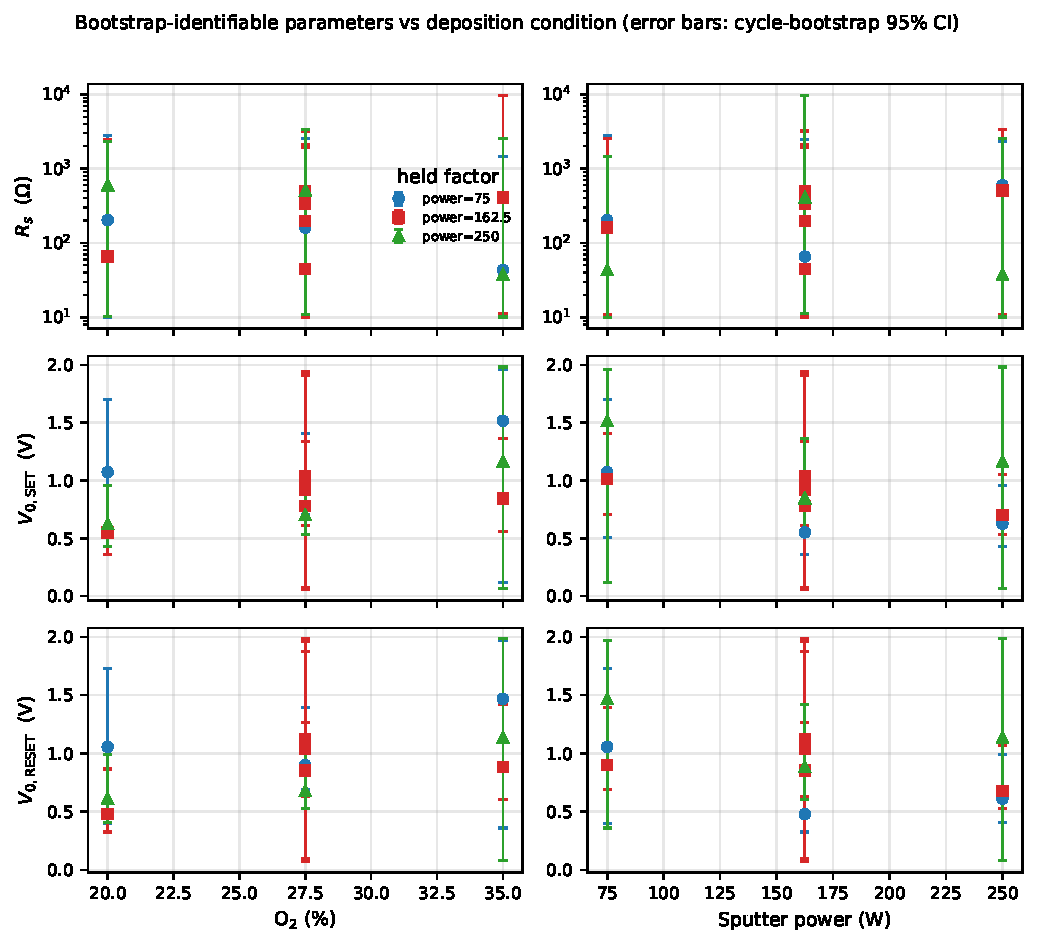
\includegraphics[width=\columnwidth]{results/paper_alt/deposition_trends.pdf}
\caption{Bootstrap-identifiable parameters versus deposition condition (error
bars: cycle-bootstrap 95\% CI).  Branch voltage scales (middle, bottom rows)
are tightly constrained and carry deposition information; series resistance
(top) spans up to two decades and cannot support a response surface despite
being locally Fisher-identifiable.}
\label{fig:trends}
\end{figure}

Finally, the regime classifier yields a device-wide, physically interpretable
HRS observable.  Figure~\ref{fig:schottky} plots the dynamic relative
permittivity implied by the post-RESET Schottky window for every condition.
All twelve values fall in the physically admissible range 4.7--32, confirming
that the dominant HRS conduction is interface-limited Schottky emission across
the entire DOE, not a fitting artifact of a single device.  The $\sim$3-fold
scatter of $\varepsilon_r^{\mathrm{dyn}}$ across the four nominally identical
center-point devices (S9--S12) indicates that the interface response itself
varies cycle to cycle and device to device, rather than being a tight function
of the nominal deposition setpoint---an automated, quantitative version of the
mechanism analysis previously performed by hand \cite{chowdhury2025mwscas}.

\begin{figure}[!t]
\centering
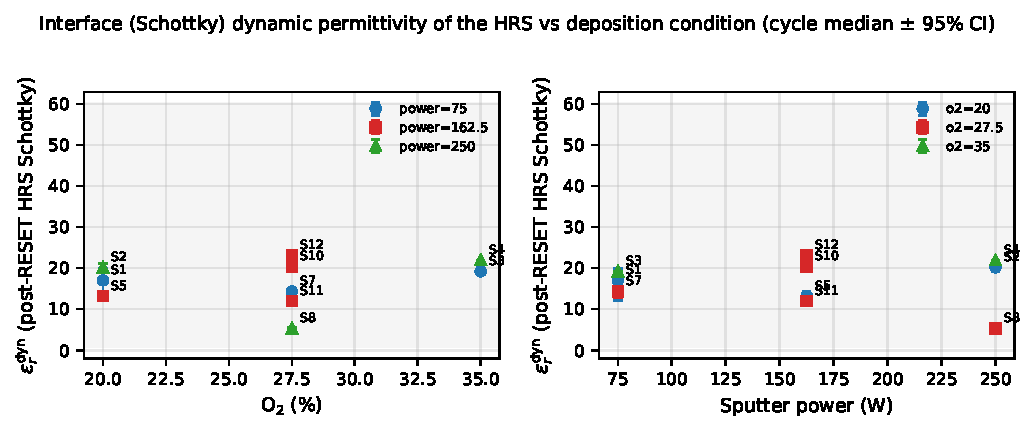
\includegraphics[width=\columnwidth]{results/paper_alt/hrs_schottky_trend.pdf}
\caption{Dynamic relative permittivity inferred from the post-RESET HRS
Schottky window for all twelve conditions, versus oxygen (left) and power
(right).  Shaded band: admissibility interval $[1,60]$.  All conditions are
physically admissible, corroborating interface-limited HRS conduction
device-wide.}
\label{fig:schottky}
\end{figure}

% =========================================================================
\section{Discussion}
\label{sec:discussion}
% =========================================================================

\subsection{Implications for Compact-Model Users}

For circuit designers consuming calibrated Stanford parameter sets, the
practical messages are direct.  (i)~The calibration \emph{generalizes}: a
parameter set fitted to one representative cycle predicts the other measured
cycles of that device with the same error, so per-condition files are usable
behavioral models for the fitted protocol.  (ii)~Only the
\emph{identifiable, repeatable} combinations transfer with evidential support;
do not ascribe physical meaning to fitted $E_a$, $\nu_0$, or gap geometry from
DC sweeps alone, and do not trust a coordinate's small local uncertainty
($R_s$) without checking its bootstrap repeatability.  (iii)~When comparing
parameters across deposition conditions, compare the admissible combinations
(branch voltage scales, switching thresholds), as in
Section~\ref{sec:res-trends}, rather than raw parameter columns that mix data-
and prior-driven coordinates.

\subsection{Model Adequacy for TaO$_x$}

The regime analysis localizes the Stanford model's structural limitation for
these devices: HRS conduction is interface-limited (Schottky) in nearly all
cycles, while the model's single $\sinh$ current law is bulk-like.  This
mismatch, not optimizer failure, sets the residual floor of
Table~\ref{tab:fitquality}, as confirmed by the near-identical aggregate
unweighted RMSE of the three optimized ablation arms \emph{and} by the
out-of-sample test, in which the RESET error is elevated identically in and
out of sample.  A principled extension would add a barrier-limited HRS current
branch (or a gap-dependent barrier term)
\cite{chiu2014,bocquet2014,bengel2020jart}; the regime map produced here
provides exactly the windows and slopes such an extension should target.
Until then, down-weighting unmodelable windows during fitting prevents
interface physics from contaminating bulk parameters while keeping the
mismatch visible in unweighted validation.

\subsection{Limitations}

The transient replay is quasi-static, so kinetic parameters absorb the
effective time scale; constraining kinetics requires pulsed or
sweep-rate-resolved data \cite{ielmini2016}.  Identifiability rests on the
combined out-of-sample and bootstrap evidence, with Fisher used only as a
local cross-check and a partial set of profile-likelihood scans (S1--S4) as
corroboration; a future release should complete profile likelihood at one
common optimum for all conditions.  The bootstrap and out-of-sample analyses
are cycle-level for one selected device per condition and therefore quantify
cycle-to-cycle, not device-to-device or wafer-level, variability---although
the four replicated center-point conditions give a first indication of
device-to-device spread.  Finally, the reset-side $\gamma_0$ is structurally
overridden under negative bias in the released Verilog-A, so it is retained
for model compatibility but not physically interpreted.

% =========================================================================
\section{Conclusion}
\label{sec:conclusion}
% =========================================================================

We presented an identifiability-aware pipeline that fits the Stanford RRAM
compact model to measured TaO$_x$ DC switching data and reports, with every
parameter set, the evidence behind it.  Applied uniformly to twelve
sputter-deposition conditions, the flow achieves mean RMSE of 0.530 (SET) and
0.761 (RESET) decades and establishes findings that overlay plots alone
cannot.  First, the single-cycle calibration generalizes: scored against all
other measured cycles, its held-out median RMSE (0.542/0.800 decades) matches
the in-sample value to within 0.04 decades, so the fit reflects the device
rather than the chosen target.  Second, cycle-bootstrap analysis shows that
only the branch voltage scales are repeatable, while series resistance and
velocity prefactors are not---and that a coordinate's small \emph{local}
Fisher uncertainty (e.g.\ $R_s$) does not imply repeatability.  Consequently,
only the identifiable, repeatable combinations carry usable deposition
information across the DOE.  Third, the post-RESET HRS is Schottky-limited in
92.5--100\% of cycles for every condition, with physically admissible
permittivities, a mechanism outside the Stanford bulk current law that bounds
achievable fidelity.  Generalization, identifiability, and mechanism validity
should therefore be reported together as the deliverable of RRAM
compact-model calibration.

% =========================================================================
\begin{thebibliography}{99}\footnotesize

\bibitem{wong2012metal}
H.-S.~P. Wong \emph{et~al.}, ``Metal-oxide RRAM,'' \emph{Proc. IEEE},
vol.~100, no.~6, pp. 1951--1970, Jun. 2012.

\bibitem{ielmini2018inmemory}
D.~Ielmini and H.-S.~P. Wong, ``In-memory computing with resistive switching
devices,'' \emph{Nature Electron.}, vol.~1, pp. 333--343, 2018.

\bibitem{yu2018neuro}
S.~Yu, ``Neuro-inspired computing with emerging nonvolatile memories,''
\emph{Proc. IEEE}, vol.~106, no.~2, pp. 260--285, Feb. 2018.

\bibitem{guan2012spice}
X.~Guan, S.~Yu, and H.-S.~P. Wong, ``A SPICE compact model of metal oxide
resistive switching memory with variations,'' \emph{IEEE Electron Device
Lett.}, vol.~33, no.~10, pp. 1405--1407, Oct. 2012.

\bibitem{jiang2016verification}
Z.~Jiang \emph{et~al.}, ``A compact model for metal--oxide resistive random
access memory with experiment verification,'' \emph{IEEE Trans. Electron
Devices}, vol.~63, no.~5, pp. 1884--1892, May 2016.

\bibitem{bocquet2014}
M.~Bocquet \emph{et~al.}, ``Robust compact model for bipolar oxide-based
resistive switching memories,'' \emph{IEEE Trans. Electron Devices}, vol.~61,
no.~3, pp. 674--681, Mar. 2014.

\bibitem{bengel2020jart}
C.~Bengel \emph{et~al.}, ``Variability-aware modeling of filamentary
oxide-based bipolar resistive switching cells using SPICE level compact
models,'' \emph{IEEE Trans. Circuits Syst. I, Reg. Papers}, vol.~67, no.~12,
pp. 4618--4630, Dec. 2020.

\bibitem{kvatinsky2015vteam}
S.~Kvatinsky \emph{et~al.}, ``VTEAM: A general model for voltage-controlled
memristors,'' \emph{IEEE Trans. Circuits Syst. II, Exp. Briefs}, vol.~62,
no.~8, pp. 786--790, Aug. 2015.

\bibitem{transtrum2015sloppiness}
M.~K. Transtrum \emph{et~al.}, ``Perspective: Sloppiness and emergent theories
in physics, biology, and beyond,'' \emph{J. Chem. Phys.}, vol. 143, no.~1,
Art. no. 010901, 2015.

\bibitem{gutenkunst2007}
R.~N. Gutenkunst \emph{et~al.}, ``Universally sloppy parameter sensitivities in
systems biology models,'' \emph{PLoS Comput. Biol.}, vol.~3, no.~10,
pp. 1871--1878, 2007.

\bibitem{raue2009}
A.~Raue \emph{et~al.}, ``Structural and practical identifiability analysis of
partially observed dynamical models by exploiting the profile likelihood,''
\emph{Bioinformatics}, vol.~25, no.~15, pp. 1923--1929, 2009.

\bibitem{chis2011}
O.-T. Chis, J.~R. Banga, and E.~Balsa-Canto, ``Structural identifiability of
systems biology models: A critical comparison of methods,'' \emph{PLoS ONE},
vol.~6, no.~11, Art. no. e27755, 2011.

\bibitem{chiu2014}
F.-C. Chiu, ``A review on conduction mechanisms in dielectric films,''
\emph{Adv. Mater. Sci. Eng.}, vol. 2014, Art. no. 578168, 2014.

\bibitem{ielmini2016}
D.~Ielmini, ``Resistive switching memories based on metal oxides: Mechanisms,
reliability and scaling,'' \emph{Semicond. Sci. Technol.}, vol.~31, no.~6,
Art. no. 063002, 2016.

\bibitem{wouters2015}
D.~J. Wouters, R.~Waser, and M.~Wuttig, ``Phase-change and redox-based
resistive switching memories,'' \emph{Proc. IEEE}, vol.~103, no.~8,
pp. 1274--1288, Aug. 2015.

\bibitem{snoek2012practical}
J.~Snoek, H.~Larochelle, and R.~P. Adams, ``Practical Bayesian optimization
of machine learning algorithms,'' in \emph{Proc. Adv. Neural Inf. Process.
Syst. (NeurIPS)}, 2012, pp. 2951--2959.

\bibitem{shahriari2016}
B.~Shahriari \emph{et~al.}, ``Taking the human out of the loop: A review of
Bayesian optimization,'' \emph{Proc. IEEE}, vol.~104, no.~1, pp. 148--175,
Jan. 2016.

\bibitem{efron1994bootstrap}
B.~Efron and R.~J. Tibshirani, \emph{An Introduction to the Bootstrap}.
New York, NY, USA: Chapman \& Hall/CRC, 1994.

\bibitem{chowdhury2025mwscas}
M.~T.~R. Chowdhury, A.~Moazzeni, and G.~Tutuncuoglu, ``Atomic-scale insights
into the switching mechanisms of RRAM devices,'' in \emph{Proc. IEEE 68th
Int. Midwest Symp. Circuits Syst. (MWSCAS)}, Lansing, MI, USA, 2025,
pp. 518--522.

\bibitem{moazzeni2023}
A.~Moazzeni, M.~T.~R. Chowdhury, and G.~Tutuncuoglu, ``The impact of
operation conditions on potentiation, depression and endurance dynamics of
tantalum oxide RRAMs,'' in \emph{Proc. IEEE Int. Integr. Rel. Workshop
(IIRW)}, 2023.

\bibitem{lee2011fast}
M.-J. Lee \emph{et~al.}, ``A fast, high-endurance and scalable non-volatile
memory device made from asymmetric Ta$_2$O$_{5-x}$/TaO$_{2-x}$ bilayer
structures,'' \emph{Nature Mater.}, vol.~10, pp. 625--630, 2011.

\end{thebibliography}

\end{document}
